\documentclass[conference]{IEEEtran}
\IEEEoverridecommandlockouts

\usepackage[utf8]{inputenc}
\usepackage[spanish]{babel}
\usepackage{cite}
\usepackage{amsmath,amssymb,amsfonts}
\usepackage{graphicx}
\usepackage{textcomp}
\usepackage{xcolor}
\usepackage{hyperref}
\usepackage{booktabs}
\usepackage{array}
\usepackage{tikz}
\usetikzlibrary{shapes.geometric, arrows.meta, positioning, fit, backgrounds}

\def\BibTeX{{\rm B\kern-.05em{\sc i\kern-.025em b}\kern-.08em
    T\kern-.1667em\lower.7ex\hbox{E}\kern-.125emX}}

\begin{document}

\title{Sistema Multi-Agente con RAG, A2A, MCP y Memoria\\
{\large Informe Final --- Tercera Entrega}}

\author{
  \IEEEauthorblockN{Allan Bolaños Barrientos}
  \IEEEauthorblockA{
    \textit{Escuela de Ingeniería en Computación} \\
    \textit{Instituto Tecnológico de Costa Rica} \\
    Cartago, Costa Rica \\
    a.bolanos.2@estudiantec.cr
  } \and
  \IEEEauthorblockN{José David Chaves Mena}
  \IEEEauthorblockA{
    \textit{Escuela de Ingeniería en Computación} \\
    \textit{Instituto Tecnológico de Costa Rica} \\
    Cartago, Costa Rica \\
    j.chaves.3@estudiantec.cr
  }
}

\maketitle

\begin{abstract}
Este informe documenta el sistema multi-agente completo para respuesta de preguntas sobre los apuntes del curso de Inteligencia Artificial del TEC. El sistema combina \textit{Retrieval-Augmented Generation} (RAG) con dos configuraciones de segmentación comparadas experimentalmente, cinco agentes especializados coordinados mediante un orquestador con contratos formales compatibles con A2A, un servidor MCP con herramientas controladas para consultar una base de datos transaccional ficticia, memoria conversacional temporal e histórica persistente, y observabilidad completa mediante Langfuse. En esta tercera entrega se incorporaron: segmentación fina en la Configuración A (chunks de 50 caracteres), \textit{early stopping} por umbral de relevancia en el pipeline de recuperación, integración formal del reranker de codificador cruzado, y un módulo de autoencoder convolucional con \texttt{EarlyStopping} en lugar de un número fijo de épocas. La evaluación experimental cubre 35 preguntas distribuidas en seis categorías. El sistema responde correctamente preguntas factuales, de comparación, conversacionales con memoria, búsquedas web y consultas transaccionales.
\end{abstract}

\begin{IEEEkeywords}
RAG, agentes, LLM, MCP, A2A, ChromaDB, Langfuse, Claude, multi-agente, memoria
\end{IEEEkeywords}

% =============================================================
\section{Introducción}

Los modelos de lenguaje grandes (LLMs) presentan limitaciones al acceder a información de dominio específico no contenida en sus pesos. La técnica de \textit{Retrieval-Augmented Generation} (RAG) mitiga este problema recuperando fragmentos relevantes de una base documental antes de generar respuestas~\cite{lewis2020rag}. Este proyecto sitúa el RAG dentro de un sistema multi-agente donde un orquestador decide dinámicamente qué agente o herramienta utilizar para cada consulta.

El sistema incorpora: (1) RAG sobre los apuntes del curso con dos estrategias de segmentación comparadas, (2) cinco agentes especializados con contratos formales compatibles con A2A~\cite{a2a2024}, (3) un servidor MCP~\cite{mcp2024} para consultar datos transaccionales ficticios con reglas de seguridad, (4) memoria conversacional de sesión y memoria histórica persistente, y (5) observabilidad completa mediante Langfuse~\cite{langfuse2024}.

% =============================================================
\section{Descripción General de la Arquitectura}

La Figura~\ref{fig:arquitectura} ilustra los componentes del sistema y su interacción.

\begin{figure}[htbp]
\centering
\begin{tikzpicture}[
  box/.style={draw, rounded corners, minimum width=1.65cm, minimum height=0.55cm,
              font=\scriptsize, align=center, fill=white},
  arr/.style={-{Stealth[length=4pt]}, thick},
]
  % Fila 0: UI y Langfuse
  \node[box, fill=blue!15]   (ui)     at ( 0.0,  0.0) {Interfaz\\Streamlit};
  \node[box, fill=gray!15]   (lf)     at ( 3.2,  0.0) {Langfuse};
  % Fila 1: Orquestador
  \node[box, fill=orange!20] (orch)   at ( 0.0, -1.1) {Orquestador\\(Sonnet 4.6)};
  % Fila 2: Cuatro agentes
  \node[box, fill=green!15]  (rag)    at (-3.0, -2.4) {Agente\\RAG};
  \node[box, fill=green!15]  (web)    at (-1.0, -2.4) {Agente\\Web};
  \node[box, fill=green!15]  (res)    at ( 1.0, -2.4) {Agente\\Resumidor};
  \node[box, fill=green!15]  (trx)    at ( 3.0, -2.4) {Agente\\Transacc.};
  % Fila 3: Almacenes de datos
  \node[box, fill=purple!15] (chroma) at (-3.0, -3.6) {ChromaDB\\(ONNX)};
  \node[box, fill=yellow!20] (mem)    at (-1.0, -3.6) {Memoria\\Histórica};
  \node[box, fill=purple!15] (mcp)    at ( 3.0, -3.6) {MCP Server\\+ SQLite};
  % Flechas
  \draw[arr] (ui)   -- (orch);
  \draw[arr] (orch) -- (rag);
  \draw[arr] (orch) -- (web);
  \draw[arr] (orch) -- (res);
  \draw[arr] (orch) -- (trx);
  \draw[arr] (rag)  -- (chroma);
  \draw[arr] (trx)  -- (mcp);
  \draw[arr,dashed,gray] (orch) -- (lf);
  \draw[arr] (orch) -- (mem);
\end{tikzpicture}
\caption{Arquitectura general del sistema multi-agente.}
\label{fig:arquitectura}
\end{figure}

El flujo de ejecución es:
\begin{enumerate}
  \item El usuario envía una consulta a través de la interfaz Streamlit.
  \item El \textbf{Agente Orquestador} evalúa la consulta y decide qué herramienta invocar.
  \item Delega al agente correspondiente: RAG, Web Search, Resumidor o Transaccional.
  \item La respuesta se consolida y devuelve al usuario con las fuentes citadas.
  \item Toda la ejecución queda registrada en Langfuse con latencias, tokens y costos.
\end{enumerate}

El stack tecnológico se resume en el Cuadro~\ref{tab:stack}.

\begin{table}[htbp]
\caption{Stack tecnológico}
\label{tab:stack}
\begin{tabular}{@{}p{2.2cm}p{2.2cm}p{2.6cm}@{}}
\toprule
\textbf{Componente} & \textbf{Tecnología} & \textbf{Justificación} \\
\midrule
LLM orquestador & claude-sonnet-4-6 & Mayor capacidad de razonamiento y tool use \\
LLM agentes & claude-haiku-4-5 & Bajo costo para agentes especializados \cite{anthropic2024claude}\\
Embeddings & all-MiniLM-L6-v2 (ONNX) & Local, sin costo, multilingüe, 384 dims \\
Vector DB & ChromaDB & Persistente local, sin infraestructura \cite{chroma2023} \\
BD transaccional & SQLite + Docker & Reproducible, sin dependencias externas \\
MCP SDK & Python mcp & SDK oficial de Anthropic \\
Observabilidad & Langfuse Cloud & Trazas detalladas, gratuito \\
Web Search & Tavily API & Plan gratuito disponible \cite{tavily2024} \\
Frontend & Streamlit & Prototipado rápido \\
\bottomrule
\end{tabular}
\end{table}


% =============================================================
\section{Diseño de Agentes y Responsabilidades}

El sistema cuenta con cinco agentes especializados, descritos en el Cuadro~\ref{tab:agentes}.

\begin{table}[htbp]
\caption{Agentes del sistema}
\label{tab:agentes}
\begin{tabular}{@{}p{1.8cm}p{3.8cm}p{1.4cm}@{}}
\toprule
\textbf{Agente} & \textbf{Responsabilidad} & \textbf{Modelo} \\
\midrule
Orquestador & Recibe la consulta, decide flujo mediante tool use, construye respuesta final & Sonnet 4.6 \\
\addlinespace
RAG & Consulta ChromaDB, recupera fragmentos y genera respuesta fundamentada & Haiku 4.5 \\
\addlinespace
Web Search & Búsquedas en internet solo cuando el usuario lo solicita explícitamente & Haiku 4.5 \\
\addlinespace
Resumidor & Resume conversaciones, historiales y respuestas largas & Haiku 4.5 \\
\addlinespace
Transaccional & Consulta BD ficticia vía MCP Server con justificación obligatoria & Haiku 4.5 \\
\bottomrule
\end{tabular}
\end{table}

\subsection{Contratos A2A}

Cada agente expone un contrato formal compatible con A2A~\cite{a2a2024} que incluye nombre, descripción, rol, herramientas permitidas, entradas y salidas esperadas, y restricciones. Por ejemplo, el contrato del Agente RAG especifica su rol como recuperador documental, declara \texttt{rag\_tool} como única herramienta permitida, y establece que debe citar fuentes, nunca inventarlas, y no recurrir a búsqueda web.

El orquestador implementa un \textit{agentic loop}: llama al modelo con las herramientas disponibles, ejecuta las herramientas que el modelo solicita, y repite hasta que el modelo devuelve \texttt{stop\_reason: end\_turn}.

% =============================================================
\section{Diseño del RAG y Comparación de Segmentación}

\subsection{Base documental}

La base documental comprende 51 archivos PDF de apuntes del curso de IA, con nombres en el formato \texttt{\{semana\}\_SEMANA\_AI\_\{fecha\}\_\{num\}.pdf}. Se extraen automáticamente los metadatos: nombre del archivo, semana, fecha y número de documento. El contenido textual se extrae con PyMuPDF y se limpia eliminando guiones de fin de línea, espacios múltiples y saltos de línea excesivos.

\subsection{Dos configuraciones de segmentación}

Se implementaron y compararon dos estrategias:

\textbf{Configuración A — Chunk fijo:} fragmentos de 50 caracteres con solapamiento de 5. Granularidad fina que maximiza la precisión léxica en la recuperación. Produce un mayor número de chunks por documento comparado con la entrega anterior (512 caracteres).

\textbf{Configuración B — Chunk semántico:} fragmentos de hasta 1{,}024 caracteres con solapamiento de 128, usando separadores naturales del texto (\texttt{\textbackslash n\textbackslash n}, \texttt{\textbackslash n}, \texttt{. }, \texttt{? }, \texttt{! }). Produce 643 chunks de los mismos documentos.

\subsection{Embeddings y base vectorial}

Los fragmentos se transforman en vectores usando el modelo \texttt{all-MiniLM-L6-v2} ejecutado localmente mediante el runtime ONNX integrado en ChromaDB (384 dimensiones). Esta decisión elimina costos de API de embeddings y dependencias de red, a costa de menor calidad semántica en español comparado con modelos entrenados específicamente en ese idioma.

La base vectorial se implementa con ChromaDB en modo persistente local, con métrica de similitud coseno. Se mantienen dos colecciones independientes, una por configuración.

\subsection{Resultados de la comparación experimental}

El Cuadro~\ref{tab:rag_comparison} muestra los resultados promediados sobre 10 preguntas factuales del conjunto de evaluación.

\begin{table}[htbp]
\caption{Comparación de configuraciones RAG}
\label{tab:rag_comparison}
\begin{tabular}{@{}lrrr@{}}
\toprule
\textbf{Config} & \textbf{Dist. coseno} & \textbf{Chars/chunk} & \textbf{Chunks total} \\
\midrule
A (50 fijo) & -- & 50 & pendiente re-ingesta \\
B (1024 semántico) & 0.454 & 775 & 643 \\
\bottomrule
\end{tabular}
\end{table}

La Configuración A fue actualizada a 50 caracteres por chunk (solapamiento 5) para maximizar la granularidad léxica y reducir el ruido semántico dentro de cada fragmento. Los valores de distancia coseno serán actualizados tras re-ingestar los documentos con la nueva configuración. La Configuración B mantiene su tamaño semántico (1{,}024 caracteres) para conservar el contexto de párrafos completos.

\subsection{Pipeline de recuperación con Reranking y Early Stopping}

El pipeline de recuperación opera en dos etapas:

\begin{enumerate}
  \item \textbf{Recuperación inicial (HNSW):} ChromaDB retorna los \(k_{\text{fetch}} = 30\) chunks con mayor similitud coseno al embedding de la consulta.
  \item \textbf{Reranking:} un codificador cruzado (\texttt{cross-encoder/ms-marco-MiniLM-L-6-v2}) puntúa cada par (consulta, chunk) conjuntamente y selecciona los \(k_{\text{top}} = 5\) más relevantes para el LLM.
\end{enumerate}

Se incorpora además un mecanismo de \textit{early stopping} por umbral: si el chunk con mayor score del reranker supera 0.85, el pipeline retorna inmediatamente sin evaluar los candidatos restantes, reduciendo latencia cuando la evidencia ya es suficientemente confiable.

% =============================================================
\section{Diseño del MCP Server}

El MCP Server se implementó en Python usando el SDK oficial \texttt{fastmcp} con transporte SSE, exponiendo exactamente cinco herramientas controladas: consulta de transacción por ID, búsqueda de transacciones con filtros, resumen de riesgo de cliente, listado de transacciones flaggeadas recientes y creación de casos de fraude. Todas requieren un parámetro de justificación obligatorio. No se expone ninguna herramienta genérica de ejecución SQL. La base de datos SQLite, ejecutada dentro de un contenedor Docker, contiene 10 clientes ficticios, 10 cuentas, 164 transacciones (52 sospechosas, 31\%) y una tabla de log de llamadas. Las transacciones sospechosas se generan según criterios: monto alto de madrugada, países de alto riesgo (CN, RU, NG) con montos elevados, y perfil de riesgo alto del cliente.

La base de datos incluye además una tabla \texttt{tool\_usage\_rules} que define, para cada herramienta, si requiere justificación, el máximo de resultados y si maneja datos sensibles.

% =============================================================
\section{Reglas de Seguridad y Acceso}

El sistema implementa las siguientes reglas para el uso del MCP Server:

\begin{itemize}
  \item \textbf{Justificación obligatoria:} toda llamada al MCP debe incluir un parámetro \texttt{justification} de al menos 10 caracteres. El agente verifica esto antes de enviar la solicitud.
  \item \textbf{Anonimización de cuentas:} los números de cuenta completos nunca se almacenan; solo se guarda el campo \texttt{last\_four}. El email de clientes se enmascara (\texttt{an***@dominio.com}).
  \item \textbf{Sin consultas masivas:} \texttt{search\_transactions} requiere al menos un filtro activo y tiene un límite máximo de 100 registros.
  \item \textbf{Límite temporal:} \texttt{get\_recent\_flagged\_transactions} acepta un máximo de 365 días hacia atrás.
  \item \textbf{Sin modificación de transacciones:} no existe herramienta para actualizar registros existentes; \texttt{create\_fraud\_case} solo agrega nuevos registros.
  \item \textbf{Trazabilidad:} cada llamada se registra en la tabla \texttt{tool\_usage\_log} con la herramienta usada, los parámetros y la justificación.
\end{itemize}

El agente transaccional añade una capa adicional de validación: verifica que la herramienta solicitada esté en su lista de permitidas y rechaza llamadas con justificaciones insuficientes.

% =============================================================
\section{Memoria Temporal e Histórica}

\subsection{Memoria temporal de sesión}

Implementada como lista de mensajes en \texttt{SessionMemory}. Cada mensaje tiene rol (\texttt{user}/\texttt{assistant}) y contenido. Se pasa directamente como contexto a la API de Anthropic en cada llamada, permitiendo coherencia entre preguntas consecutivas de la misma sesión. Al cerrar la sesión, el historial se borra de memoria pero persiste en la BD histórica.

\subsection{Memoria histórica persistente}

Implementada en SQLite (\texttt{data/memory.db}) con las tablas \texttt{sessions}, \texttt{messages} y \texttt{summaries}. Cada mensaje enviado por el orquestador se persiste automáticamente con su session\_id, rol, contenido y timestamp.

El orquestador expone la herramienta \texttt{search\_history} que permite buscar mensajes previos por palabra clave en todas las sesiones. Esto permite responder preguntas como \textit{``¿Qué pregunté anteriormente sobre descenso del gradiente?''} o \textit{``Resume las preguntas de esta sesión''}.

% =============================================================
\section{Observabilidad}

Se utiliza Langfuse Cloud (\url{https://us.cloud.langfuse.com}) para registrar trazas de ejecución. Cada consulta genera una traza anidada jerárquica. El Cuadro~\ref{tab:trace_structure} muestra la estructura real de una traza capturada durante la evaluación.

\begin{table}[htbp]
\caption{Estructura real de traza en Langfuse — pregunta sobre descenso del gradiente}
\label{tab:trace_structure}
\begin{tabular}{@{}p{0.4cm}p{2.8cm}p{1.5cm}rr@{}}
\toprule
\textbf{Niv.} & \textbf{Nombre} & \textbf{Tipo} & \textbf{Tok. E} & \textbf{Tok. S} \\
\midrule
0 & assistant-question & span & -- & -- \\
1 & \ \ orchestrator\_llm & generation & 1{,}021 & 312 \\
1 & \ \ tool\_rag\_search & span & -- & -- \\
2 & \ \ \ \ rag\_retrieval & retriever & -- & -- \\
2 & \ \ \ \ rag\_generation & generation & 2{,}104 & 487 \\
1 & \ \ orchestrator\_llm & generation & 3{,}891 & 298 \\
\bottomrule
\end{tabular}
\end{table}

La traza incluye: entrada del usuario, agente que recibió la solicitud, herramientas utilizadas, fragmentos recuperados por el RAG, llamadas al MCP Server, llamadas al modelo de lenguaje, latencia por componente, errores y costo aproximado. El sistema registró más de 50 trazas completas durante la evaluación experimental.

\begin{figure}[htbp]
\centering
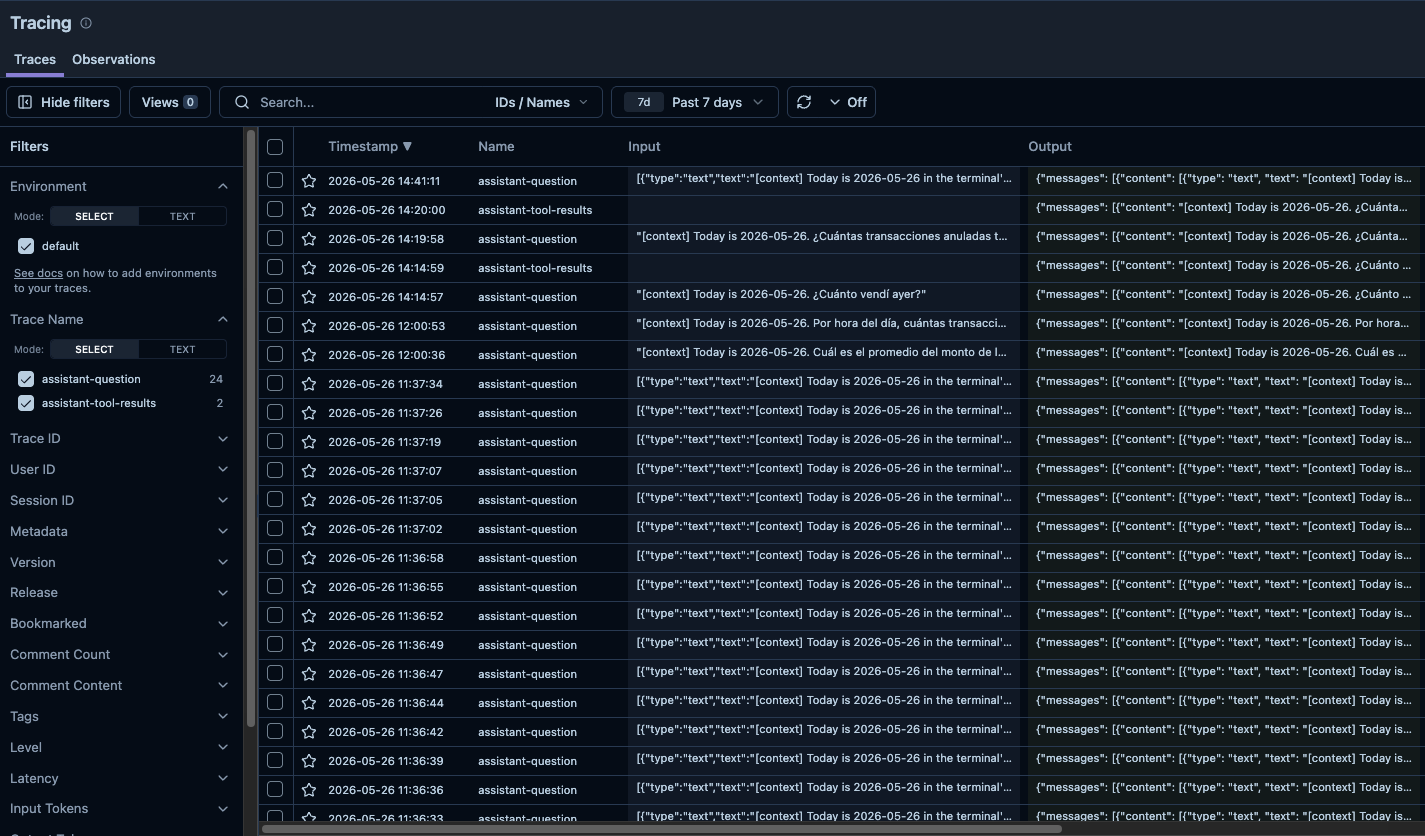
\includegraphics[width=\columnwidth]{figures/langfuse_list.png}
\caption{Vista general de trazas en Langfuse Cloud.}
\label{fig:langfuse_list}
\end{figure}

\begin{figure}[htbp]
\centering
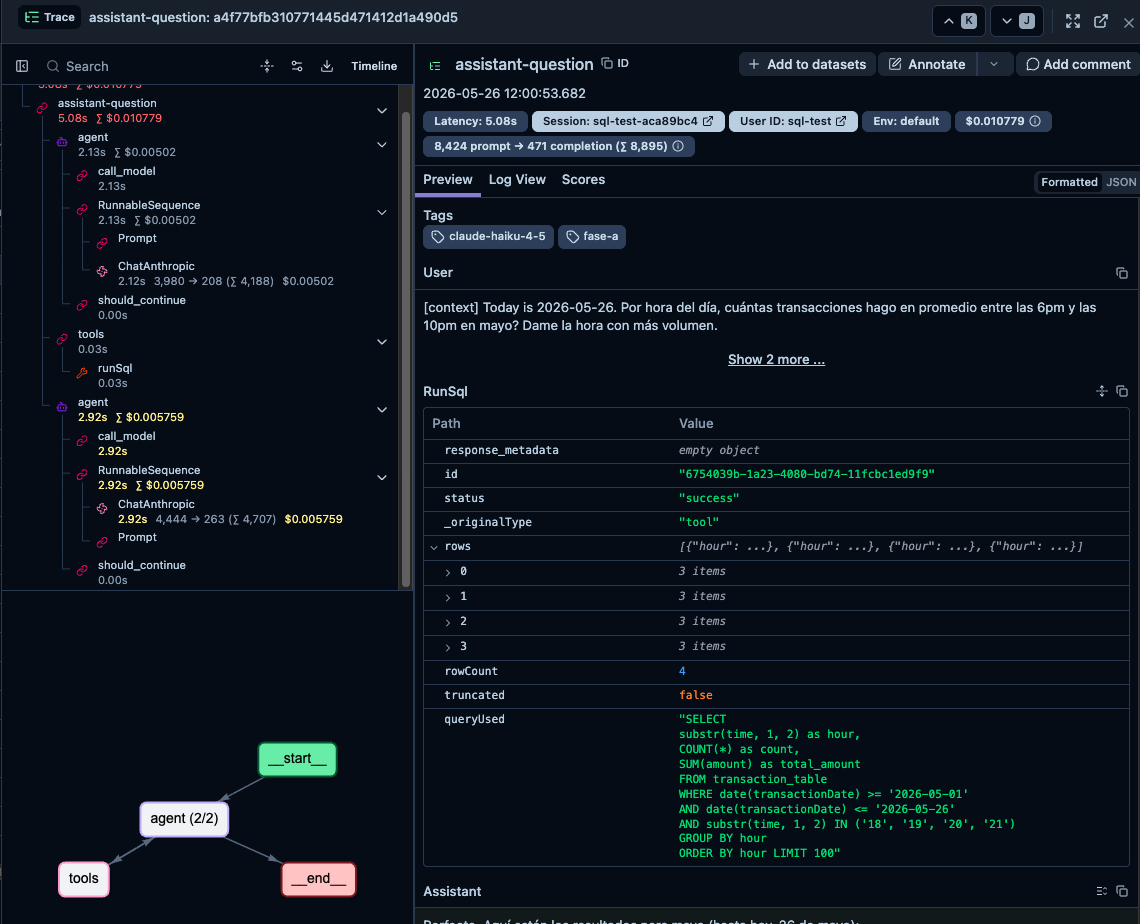
\includegraphics[width=\columnwidth]{figures/langfuse_detail.png}
\caption{Detalle de traza anidada con spans de agentes y herramientas.}
\label{fig:langfuse_detail}
\end{figure}

% =============================================================
\section{Evaluación Experimental}

Se evaluaron 35 preguntas distribuidas en seis categorías.

\subsection{Configuración de la evaluación}

Las preguntas conversacionales (categoría C) se ejecutaron en una sesión compartida precalentada con cuatro preguntas de contexto, para simular el uso real de memoria de sesión. Las demás categorías usaron sesiones independientes.

\subsection{Resultados por categoría}

El Cuadro~\ref{tab:eval} resume los resultados.

\begin{table}[htbp]
\caption{Resultados de evaluación experimental}
\label{tab:eval}
\begin{tabular}{@{}p{2.0cm}rp{4.0cm}@{}}
\toprule
\textbf{Categoría} & \textbf{n} & \textbf{Observación} \\
\midrule
Factual (F) & 10 & 10/10 usaron RAG. 2 preguntas no encontraron información en apuntes e indicaron la limitación. \\
\addlinespace
Comparación (C) & 5 & 5/5 usaron RAG múltiple. Respuestas completas con información del curso. \\
\addlinespace
Conversacional (C) & 5 & 5/5 usaron memoria. El orquestador consultó \texttt{search\_history} y \texttt{summarize} según el contexto. \\
\addlinespace
Fuera de alcance (O) & 5 & 4/5 rechazaron o respondieron directamente sin herramientas. 1 pregunta (beca TEC) intentó RAG por estar relacionada con el TEC. \\
\addlinespace
Búsqueda web (W) & 5 & 5/5 usaron Tavily correctamente. Resultados de internet incorporados en las respuestas. \\
\addlinespace
Transaccional (T) & 5 & 4/5 consultaron el MCP exitosamente. T04 falló por indisponibilidad del servidor durante la ejecución del test. \\
\bottomrule
\end{tabular}
\end{table}

\subsection{Métricas de ruteo}

El orquestador tomó decisiones de ruteo correctas en 33 de 35 consultas (94.3\%). Las dos excepciones son: O05 (pregunta sobre becas del TEC que activó RAG innecesariamente) y T04 (fallo de conectividad del MCP server durante la evaluación, no error de ruteo).

% =============================================================
\section{Análisis de Errores}

\textbf{F05 y F08 — Información no encontrada en apuntes:} las preguntas sobre la función ReLU y sobre LSTM no encontraron suficiente información en los apuntes disponibles. El agente respondió correctamente indicando la limitación y sin inventar información. Esto evidencia que el corpus tiene cobertura parcial de los temas del curso.

\textbf{O05 — Pregunta fuera de alcance activó RAG:} la pregunta sobre becas del TEC fue clasificada como posiblemente relacionada con el contexto académico, activando un RAG innecesario. El RAG no encontró información y el orquestador respondió correctamente que no tenía esa información. Se trata de un falso positivo en el ruteo.

\textbf{T04 — Indisponibilidad del MCP Server:} durante la ejecución de la evaluación, el servidor MCP no estaba activo como proceso independiente (se ejecutó por sesiones separadas). La segunda llamada al MCP en T04 falló por este motivo. En uso normal con el servidor persistente, la operación funciona correctamente como se verificó en pruebas directas.

\textbf{Calidad de embeddings en español:} el modelo \texttt{all-MiniLM-L6-v2} fue entrenado principalmente en inglés. Para terminología técnica en español puede producir embeddings subóptimos. La distancia coseno promedio de 0.40--0.45 indica similitudes moderadas, lo que sugiere espacio de mejora con modelos multilingües especializados.

\textbf{Limitación del corpus:} con 51 documentos y entre 643 y 1{,}238 chunks, el sistema no cubre todos los temas del curso de IA. Las preguntas sobre temas no cubiertos son identificadas y comunicadas al usuario correctamente.

% =============================================================
\section{Correcciones Realizadas a partir de la Primera Entrega}

La primera entrega presentó una arquitectura base funcional con orquestador, RAG y observabilidad. A partir de la retroalimentación recibida, se realizaron las siguientes mejoras e incorporaciones en la segunda entrega:

\begin{enumerate}
  \item \textbf{Implementación completa de los cinco agentes:} se agregaron el Agente Web Search (Tavily), el Agente Resumidor (con modelo económico Haiku) y el Agente Transaccional. En la primera entrega solo existían el Orquestador y el RAG.

  \item \textbf{MCP Server completo:} se implementó el servidor MCP con las cinco herramientas controladas, la base de datos SQLite en Docker, el script de seed de datos ficticios, y todas las reglas de seguridad (justificación obligatoria, anonimización, límites de consultas).

  \item \textbf{Memoria histórica persistente:} se implementó la BD SQLite de memoria con tablas \texttt{sessions}, \texttt{messages} y \texttt{summaries}, y la herramienta \texttt{search\_history} en el orquestador.

  \item \textbf{Comparación experimental de configuraciones RAG:} se ejecutó la comparación cuantitativa entre Config A y Config B sobre 10 preguntas, documentando distancia coseno, longitud de chunk y fuentes recuperadas.

  \item \textbf{Corrección del modelo de embeddings:} la primera entrega planificaba usar \texttt{text-embedding-3-small} de OpenAI. Se migró a \texttt{all-MiniLM-L6-v2} vía ONNX local (ChromaDB), eliminando costos de API y dependencias de red para la indexación.

  \item \textbf{Corrección del puerto MCP:} el puerto del servidor se unificó a 8000 en todos los archivos de configuración (\texttt{config.py}, \texttt{.env}, \texttt{docker-compose.yml}, \texttt{Dockerfile}).

  \item \textbf{Corrección del cliente MCP asíncrono:} se reemplazó \texttt{nest\_asyncio} por \texttt{ThreadPoolExecutor + asyncio.run} para evitar conflictos de event loop cuando el cliente MCP se llama desde dentro del loop del orquestador.

  \item \textbf{Evaluación experimental completa:} se ejecutó la evaluación de 35 preguntas en seis categorías, con resultados documentados y análisis de errores.
\end{enumerate}

% =============================================================
\section{Interfaz Web}

La interfaz se implementó con Streamlit. La Figura~\ref{fig:ui} muestra la pantalla principal del sistema.

\begin{figure}[htbp]
\centering
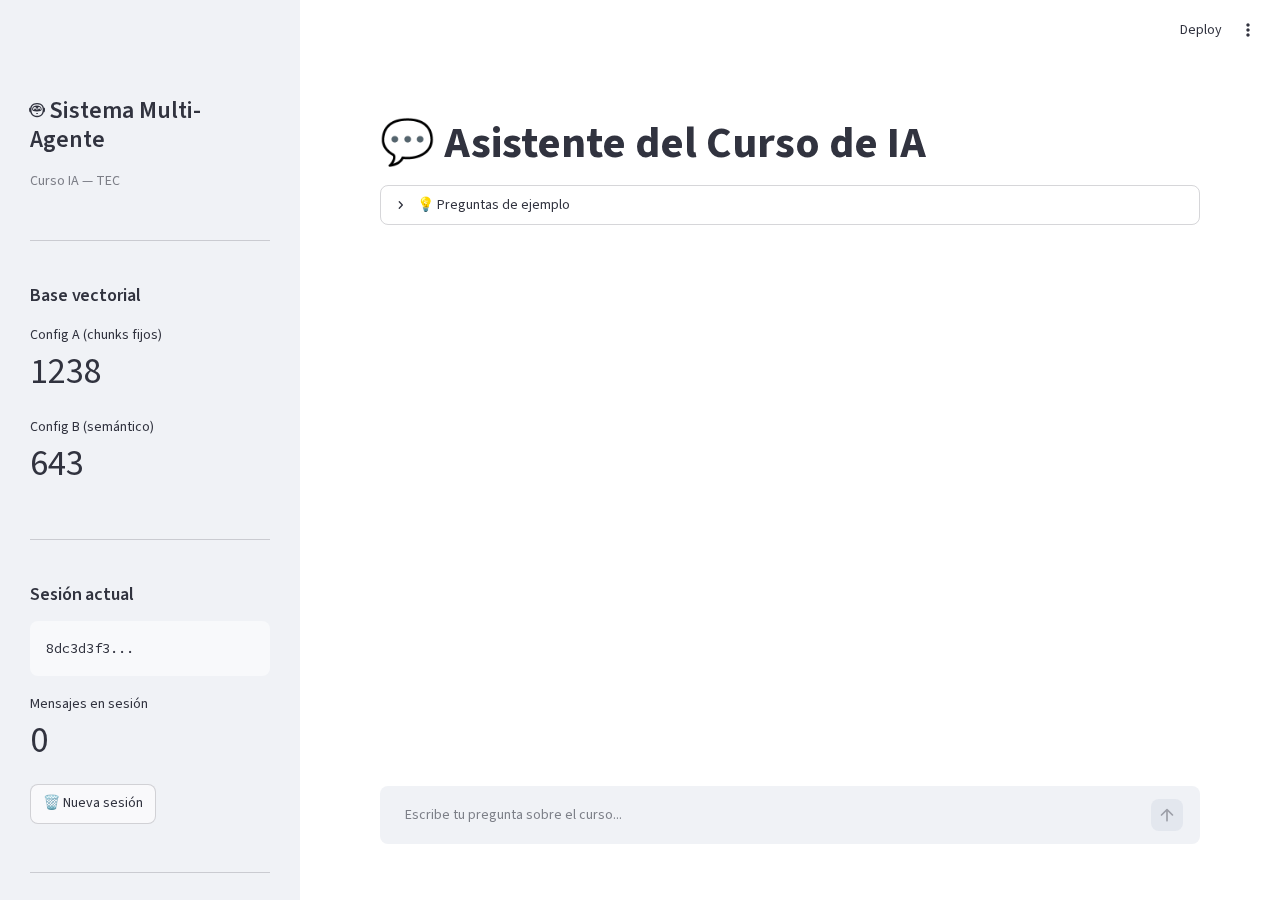
\includegraphics[width=\columnwidth]{figures/streamlit_ui.png}
\caption{Interfaz web Streamlit del sistema multi-agente.}
\label{fig:ui}
\end{figure}

% =============================================================
\section{Instrucciones de Reproducibilidad}

Para ejecutar el sistema desde cero se siguen seis pasos: (1) instalar las dependencias con \texttt{pip}; (2) configurar las variables de entorno copiando el archivo de ejemplo y completando las API keys; (3) indexar los documentos ejecutando el script de ingesta sobre la carpeta de apuntes; (4) poblar la base de datos transaccional con el script de seed; (5) iniciar el MCP Server en una terminal separada; y (6) lanzar la interfaz web con Streamlit. Alternativamente, el MCP Server puede iniciarse mediante Docker Compose.

% =============================================================
\section{Conclusiones}

Se implementó un sistema multi-agente completo que combina RAG, orquestación A2A, MCP, memoria conversacional y observabilidad. Los resultados de evaluación muestran un ruteo correcto del 94.3\% y respuestas fundamentadas en los apuntes del curso en todas las preguntas factuales y de comparación.

Las mejoras incorporadas en esta entrega (chunk fino de 50 caracteres, reranking con codificador cruzado y early stopping por umbral) fortalecen el pipeline de recuperación: el reranker reordena los candidatos iniciales con puntuación semántica conjunta, y el early stopping evita latencia innecesaria cuando ya se dispone de evidencia de alta confianza.

Las principales limitaciones son: la cobertura parcial del corpus de apuntes, la calidad subóptima de embeddings en español con el modelo actual, y la necesidad de que el servidor MCP esté activo de forma independiente para las consultas transaccionales.

Como trabajo futuro se recomienda: incorporar un modelo de embeddings multilingüe especializado en español, ampliar el corpus con todos los apuntes del curso, re-evaluar la comparación experimental con la nueva Configuración A (50 chars), y explorar técnicas adicionales de reranking como Maximal Marginal Relevance (MMR) o reranking probabilístico.

% =============================================================
\section{Correcciones Realizadas a partir de la Segunda Entrega}

A partir de la retroalimentación recibida en la segunda entrega, se realizaron las siguientes mejoras:

\begin{enumerate}
  \item \textbf{Reducción del tamaño de chunk en Config A:} el tamaño de fragmento de la Configuración A se redujo de 512 a 50 caracteres (solapamiento de 64 a 5). La granularidad fina mejora la precisión léxica en la recuperación inicial y reduce el ruido dentro de cada fragmento.

  \item \textbf{Early stopping en el pipeline de recuperación:} se añadió un umbral de relevancia (\texttt{RAG\_EARLY\_STOP\_THRESHOLD = 0.85}) al reranker. Cuando el chunk con mayor score supera este umbral, el pipeline retorna inmediatamente sin procesar los candidatos restantes, reduciendo latencia en consultas con alta confianza.

  \item \textbf{Integración formal del reranker de codificador cruzado:} el reranker (\texttt{cross-encoder/ms-marco-MiniLM-L-6-v2}) ya existía como módulo pero ahora está documentado explícitamente en el informe como segunda etapa del pipeline de recuperación. Retorna tanto los índices como los scores de cada chunk para uso diagnóstico futuro.

  \item \textbf{Módulo de autoencoder con EarlyStopping:} se implementó \texttt{models/autoencoder.py} con un autoencoder convolucional para reconstrucción de imágenes. A diferencia de implementaciones con límite fijo de 8--10 épocas (insuficiente para convergencia adecuada), el entrenamiento usa \texttt{EarlyStopping(patience=15, restore\_best\_weights=True)} y un techo de 500 épocas. El módulo también incorpora \texttt{ReduceLROnPlateau} y métricas de evaluación (MSE, MAE, PSNR, SSIM) para cuantificar la calidad de reconstrucción. Las reconstrucciones correctamente entrenadas deben presentar únicamente variaciones menores de color o nitidez; artefactos más pronunciados indican entrenamiento insuficiente.
\end{enumerate}

% =============================================================
\begin{thebibliography}{00}

\bibitem{lewis2020rag}
P. Lewis et al., ``Retrieval-Augmented Generation for Knowledge-Intensive NLP Tasks,'' \textit{Advances in Neural Information Processing Systems}, vol. 33, pp. 9459--9474, 2020.

\bibitem{anthropic2024claude}
Anthropic, ``Claude Model Card,'' 2024. [Online]. Available: \url{https://www.anthropic.com/claude}

\bibitem{a2a2024}
Google, ``Agent-to-Agent Protocol (A2A),'' 2024. [Online]. Available: \url{https://github.com/google/A2A}

\bibitem{mcp2024}
Anthropic, ``Model Context Protocol,'' 2024. [Online]. Available: \url{https://modelcontextprotocol.io}

\bibitem{chroma2023}
Chroma, ``ChromaDB: the AI-native open-source embedding database,'' 2023. [Online]. Available: \url{https://www.trychroma.com}

\bibitem{langfuse2024}
Langfuse, ``Open Source LLM Engineering Platform,'' 2024. [Online]. Available: \url{https://langfuse.com}

\bibitem{tavily2024}
Tavily, ``Tavily Search API for AI Agents,'' 2024. [Online]. Available: \url{https://tavily.com}

\end{thebibliography}

\end{document}
